\documentclass[]{article}
\usepackage{lmodern}
\usepackage{amssymb,amsmath}
\usepackage{ifxetex,ifluatex}
\usepackage{fixltx2e} % provides \textsubscript
\ifnum 0\ifxetex 1\fi\ifluatex 1\fi=0 % if pdftex
  \usepackage[T1]{fontenc}
  \usepackage[utf8]{inputenc}
\else % if luatex or xelatex
  \ifxetex
    \usepackage{mathspec}
  \else
    \usepackage{fontspec}
  \fi
  \defaultfontfeatures{Ligatures=TeX,Scale=MatchLowercase}
\fi
% use upquote if available, for straight quotes in verbatim environments
\IfFileExists{upquote.sty}{\usepackage{upquote}}{}
% use microtype if available
\IfFileExists{microtype.sty}{%
\usepackage{microtype}
\UseMicrotypeSet[protrusion]{basicmath} % disable protrusion for tt fonts
}{}
\usepackage[margin=1in]{geometry}
\usepackage{hyperref}
\hypersetup{unicode=true,
            pdfborder={0 0 0},
            breaklinks=true}
\urlstyle{same}  % don't use monospace font for urls
\usepackage{longtable,booktabs}
\usepackage{graphicx,grffile}
\makeatletter
\def\maxwidth{\ifdim\Gin@nat@width>\linewidth\linewidth\else\Gin@nat@width\fi}
\def\maxheight{\ifdim\Gin@nat@height>\textheight\textheight\else\Gin@nat@height\fi}
\makeatother
% Scale images if necessary, so that they will not overflow the page
% margins by default, and it is still possible to overwrite the defaults
% using explicit options in \includegraphics[width, height, ...]{}
\setkeys{Gin}{width=\maxwidth,height=\maxheight,keepaspectratio}
\IfFileExists{parskip.sty}{%
\usepackage{parskip}
}{% else
\setlength{\parindent}{0pt}
\setlength{\parskip}{6pt plus 2pt minus 1pt}
}
\setlength{\emergencystretch}{3em}  % prevent overfull lines
\providecommand{\tightlist}{%
  \setlength{\itemsep}{0pt}\setlength{\parskip}{0pt}}
\setcounter{secnumdepth}{5}
% Redefines (sub)paragraphs to behave more like sections
\ifx\paragraph\undefined\else
\let\oldparagraph\paragraph
\renewcommand{\paragraph}[1]{\oldparagraph{#1}\mbox{}}
\fi
\ifx\subparagraph\undefined\else
\let\oldsubparagraph\subparagraph
\renewcommand{\subparagraph}[1]{\oldsubparagraph{#1}\mbox{}}
\fi

%%% Use protect on footnotes to avoid problems with footnotes in titles
\let\rmarkdownfootnote\footnote%
\def\footnote{\protect\rmarkdownfootnote}

%%% Change title format to be more compact
\usepackage{titling}

% Create subtitle command for use in maketitle
\newcommand{\subtitle}[1]{
  \posttitle{
    \begin{center}\large#1\end{center}
    }
}

\setlength{\droptitle}{-2em}

  \title{}
    \pretitle{\vspace{\droptitle}}
  \posttitle{}
    \author{}
    \preauthor{}\postauthor{}
    \date{}
    \predate{}\postdate{}
  
\usepackage{float}
\usepackage{tikz}

\usepackage{amsthm}
\newtheorem{theorem}{Theorem}[section]
\newtheorem{lemma}{Lemma}[section]
\theoremstyle{definition}
\newtheorem{definition}{Definition}[section]
\newtheorem{corollary}{Corollary}[section]
\newtheorem{proposition}{Proposition}[section]
\theoremstyle{definition}
\newtheorem{example}{Example}[section]
\theoremstyle{definition}
\newtheorem{exercise}{Exercise}[section]
\theoremstyle{remark}
\newtheorem*{remark}{Remark}
\newtheorem*{solution}{Solution}
\begin{document}

\hypertarget{appendix-appendix}{%
\appendix}


\hypertarget{appendixA}{%
\section{Appendix: Service Order Classification}\label{appendixA}}

Service orders issued by CGU investigated different uses of public
resources in addition to procurement, e.g.~for officials compensation,
for school activities, or for community monitoring of public policies.
The discretion measure proposed here, however, is exclusive to
procurement expenditures made under Law 8,666/93. The ideal dataset for
this study would contain explicit procurement information collected by
CGU auditors, but unfortunately this is not the case. The reporting of
procurement processes is implicit, via descriptions of investigations or
findings of violations to Law 8,666/93. Thus, we isolate service orders
which investigated procurement processes from the rest by implementing
an classification system based on the information retrieval and
natural-language processing literatures.

The system uses each service order's description to identify if it is
procurement-related. In these descriptions, CGU auditors report the
purpose of their investigation, e.g.~whether they are looking into
painkiller purchases, whether the municipality has used the funds within
designated goals, or whether primary school teachers were hired for the
implementation of a school program. Using these textual descriptions as
bag-of-words models, we implement a method similar to that of Hopkins \&
King (2009): we stem and combine unigrams to form search patterns that
identify a service order as procurement-related. There are two broad
types of procurement in Law 8,666/93: (i) ordinary procurement of goods
and services, which we call \emph{purchases}; and (ii) procurement of
goods and services used for public works, which we call \emph{works}.
There are different search patterns for each type.

An example is useful for understanding our classification process.
Unigram ``aquisição'' (\emph{acquisition} in English) is stemmed to
``aquisi'' to form a search pattern for the \emph{purchases}-type
procurement; unigrams ``adequação'' and ``habitacional'' are stemmed and
combined to form ``adequa(.)*habitac''\footnote{All seach patterns are
  regular expressions.} search pattern for \emph{works}-type
procurement. This bigram picks up variations in main keywords as well as
coding mistakes due to, for instance, multiple whitespace between the
two unigrams or due to coding Portuguese special characters
(``adequação'' vs. ``adequacao'').

\textbf{Table A.1: Procurement Search Terms}

\emph{- insert table 1: keywords here -}

The final list contains 19 \emph{n}-grams for identification of
purchases and 17 \emph{n}-grams for works.\footnote{One of these
  keywords in the works search pattern is an ``exclusion keyword,''
  which removes service orders that contain the ``exclusion keyword'' in
  their description from the sample identified by the other 16
  \emph{n}-grams.} When any of these words is found, we include the
service order into the purchases or the works group. Since all public
works projects procure goods and services but not all public purchases
are works-related, whenever the search patterns matches service orders
to both groups, we include the service order only in the works group but
not in the purchases group. Public works procurements are a subset of
all public procurements in Brazilian municipalities. The search patterns
here identify a total of 9593 procurement-related service orders.

\begin{figure}[htbp]

{\centering 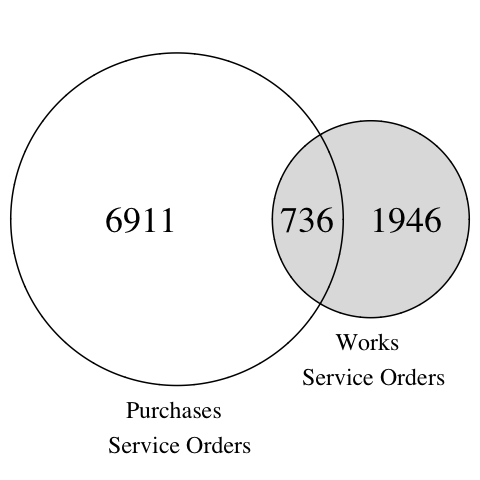
\includegraphics[width=0.3\linewidth]{venn} 

}

\caption{Sets of Procurement Service Orders}\label{fig:venn}
\end{figure}

As Grimmer \& Stewart (2013) rightly point out, no text analysis
algorithm is perfect and only relying on keyword matches could
potentially lead to misclassification of service orders. Let us suppose
that one description reads ``expenditures made in accordance with
primary education program.'' Using unigram ``expenditure'' would yield a
match for this service order to the purchases group, but in fact
auditors might be looking at bonus payments for high-performing
teachers. These resources could also be directed for school
construction. In the first case, the service order should not be have
been included in any group because it does not carry any procurement
component. In the second case, it should have also been marked as public
works.

We address these classification problems in three ways: (i) using means
comparison tests of match quality discussed in Assumpcao (2018); (ii)
comparing the performance of the same search patterns on another textual
description for a subset of service orders; (iii) finally, comparing the
results from the textual classification algorithm to that of procurement
violations reported by CGU auditors. We discuss these three tests in
turns in the following sections.

\hypertarget{quality1}{%
\subsection{Means Tests}\label{quality1}}

The first test on match quality is the means comparison test presented
in Assumpcao (2018), whose reasoning is simple. Increasing the number of
procurement-related terms in the search pattern is not necessarily good
practice as we increase the chance of misclassifying service orders as
procurement when in fact they are not; words can take on different
meanings depending on their contexts, so the more search terms we use
the more likely type I error is. Ideally, we would want to use as few
\emph{n}-grams as possible while still identifying all possible
procurement matches. In order to do this, what Assumpcao (2018) suggests
is testing match quality by incrementally comparing sample means
identified by \emph{n} vs. \emph{n} - 1 keywords. This method translates
into a check on whether the sample identified by one additional keyword
is significantly better than the previous sample with one fewer term.
The program developed by Assumpcao (2018) does this for us and we report
the results in the tables below:

\textbf{Table A.2: Purchases Search Results}

\emph{- insert table 2: Purchases Search Results here -}

The search terms are sorted in descending order by the number of service
orders they identify (column 1). Column 6 displays \emph{p}-values for
means tests across samples, where each mean is the sum of observations
found by \emph{any} of the search items before, and inclusive of, any
particular row over the total number of observations.\footnote{This is
  also known as an alternative search where all search conditions are
  connected by an ``or'' statement.} The means test thus compares
whether the sample identified by all search terms up to any row is
significantly different from the the sample identified by all rows
before. For instance, the evidence presented in row four of table 2 is
that the inclusion of search item ``ve{[}íi{]}culo'' significantly
improves (at the 5\% level) the identification of the purchases sample
when compared to the sample which only includes the previous three
search words.

\textbf{Table A.3: Works Search Results}

\emph{- insert table 3: Works Search Results here -}

The works sample is a third of the size of the purchases group and two
of its search items do not significantly identify a new sample
(``saneamento'' and ``conclus{[}ãa{]}o''). Despite having positive
individual finds reported in column 1, table A.3, the means test in
column 6 suggests that these finds are not new service orders in
addition to what had already been identified by the the previous search
terms.\footnote{The search without these terms (available upon request)
  yields 2,679 service orders, just three short of the total in table
  A.3. Nevertheless, we keep the two items in the search algorithm for
  additional tests discussed in section \ref{quality2}.}

Means tests are important to map out the relationship between search
items, both within and across groups, but they do not tell us anything
about the relationship between search items and their latent procurement
groups. In other words, the search terms might be picking up groups that
are internally consistent but that do not map onto the procurement types
in Law 8,666/93. We discuss these issues in sections \ref{quality2} and
\ref{quality3}.

\hypertarget{quality2}{%
\subsection{Textual Descriptions}\label{quality2}}

CGU service orders can best be described as investigations on the use of
public resources transferred from the federal government to Brazilian
municipalities. There are six transfer types and each service order
investigates only one type at a time. Since the procurement categories
set out in Law 8,666/93 apply to all public procurements at all
government levels, transfer types are irrelevant for constructing our
discretion measure. Nonetheless, one type of these transfers helps test
our classification algorithm.

Federal grants (\emph{convênios} in Portuguese) are narrow transfer
agreements signed by the federal government, its agencies, states and
municipalities for the delivery of governmental programs. They are
voluntary, time-limited transfers implementing policies at the local
level, such as vaccinations and the construction of community health
clinics. The most important feature of these grants, however, is that
each of them also has an individual textual description of its purpose,
e.g.~a tractor purchase for a rural community in a given municipality.
Thus, for a subset of service orders that are investigations of the use
of these federal grants by Brazilian municipalities, we have two
different textual descriptions of resource use: CGU's, from their audit
report, and the federal government's, available online at the
Transparency Portal.\footnote{\url{http://www.portaltransparencia.gov.br/}}

\textbf{Table A.4: Classification by Textual Descriptions}

\emph{- insert table 4 here -} (merge purchases and works into one
table)

There is a total of 3,868 service orders for which we have descriptions
both from CGU and from the federal government. In table A.4, we report
the results of the search algorithm both in the service order (row-wise)
and the transfer (column-wise) descriptions. We evaluate the performance
of the search algorithm by checking whether it assigns the same service
order to the same procurement group \emph{regardless of the description
in which it searches for the key terms}. In other words, the smaller the
number of times that the algorithm assigns any service order to a
different group when it switches to another textual description, the
better.

This is a particularly important point for the classification method
proposed here. The means test conducted in section \ref{quality1}
provides internal consistency because it compares and checks whether
more observations are matched when more search terms are included; the
tabulation across descriptions here provides external consistency
because it compares and checks if the classification algorithm is
independent of search target (description). It resembles a false
positive (type I error) test because we can roughly calculate the
percentage of misclassification of service orders. In panel A, the
service order description search assigns 1,556 to the purchases group,
out of which 83 were not simultaneously assigned to the same group in
the grant description search, yielding a 5.3\% false positive rate. In
panel B, the service order search marks 2,053 observations to the works
group, where 404 are not simultaneously marked when the search is
performed in the grant description (a 19.7\% type I error
rate).\footnote{The inverse misclassification rates are also reassuring:
  false positives are 8.9\% and 14.0\% for purchases and works
  respectively when we first classify observations using grant
  descriptions and then move on to service order descriptions.}

\hypertarget{quality3}{%
\subsection{Procurement Violations}\label{quality3}}

Though section \ref{quality2} supports external validity by showing that
the service order classification is consistent across textual
descriptions, we run the last robustness check here using the actual
procurement violations reported by CGU.

The findings reported by auditors are coded into 35 infractions of the
use of public resources, nine of which violations of procurement rules
and one violation of public works rules. Thus, we know with certainty
that service orders for which there are any of the nine procurement
violations (ten if public works) are in fact procurement-related and
should be classified either as purchases, works, or both. As opposed to
section \ref{quality2}, this resembles a false negative (type II error)
test on yet another subset of observations for which certain infractions
were reported.\footnote{The reason why this is a type II error test,
  instead of type I, resides on the way the test samples are defined. In
  section \ref{quality2}, both sample assignments (by matching
  procurement keywords in the service order or grant description) can be
  the ``correct'' procurement sample against which the match on the
  alternative description might yield false positives. In this section,
  we know with certainty that the sample identified by procurement
  infractions is in fact the correctly identified sample, since there
  cannot exist a procurement violation where no procurement has
  occurred. It makes the unidentified observations false negatives
  because they should have been classified as procurement-related
  service orders. This sample is clearly underidentified, as there are
  many procurement-related service orders that simply followed Law
  8,666/93 and thus carry no infraction, but still, within this subset
  of all CGU investigations, it provides us with a good conterfactual
  against which to test our classification mechanism.}

\textbf{Table A.5: Classification by Violation Code}

\emph{- insert table 5 here -} (use procurement table, not split up by
purchases or works. Explain why denominator is any procurement)

The total number of service orders with at least one procurement
infraction is 3,775 (4,146 if we include the public works infraction),
which is the sum of column 2 in table A.5, panels A and B. The false
negative rate is 8.5\% and 9.9\%, respectively, for purchases-only and
works procurements. This means that 319 and 344 service orders should
have been classified as procurement by our textual search algorithm but
were not.

Although no text analysis mechanism is perfect, the evidence presented
here supports our choice of classification algorithm. The identification
of procurement orders is internally consistent (section \ref{quality1}),
there are very few incorrect assignments of service orders to
procurement (section \ref{quality2}), and the sample which was
identified as procurement maps well onto the latent categories in the
Brazilian procurement legislation (section \ref{quality3}).

\hypertarget{appendixB}{%
\section{Appendix: Service Amount Manipulation}\label{appendixB}}

The identification strategy in this paper relies on the assumption that
municipal officials do not (completely) manipulate public expenditure
amounts in order to avoid stricter procurement rules. In other words,
the public procurement processes carried out just below and above any
discretion threshold, which is uniquely determined by procurement
amount, are equal except for the rules set out in Law 8,666/93. We
present below the McCrary (2008) test for manipulation of running
variable for all six discretion cutoffs in the Brazilian procurement
legislation.

\emph{- Insert graphics -}

These tests show that manipulation of procurement amount is not
particularly problematic except for purchases cutoff three, which is
thus excluded from the analysis.

\hypertarget{appendixC}{%
\section{Appendix: CEPESP Infraction Classification}\label{appendixC}}

\emph{- insert table - }

\hypertarget{refs}{}
\leavevmode\hypertarget{ref-AssumpcaotextfindDataDrivenText2018}{}%
Assumpcao, A. (2018). \emph{Textfind: A Data-Driven Text Analysis Tool
for Stata}.

\leavevmode\hypertarget{ref-GrimmerTextDataPromise2013a}{}%
Grimmer, J., \& Stewart, B. M. (2013). Text as Data: The Promise and
Pitfalls of Automatic Content Analysis Methods for Political Texts.
\emph{Political Analysis}, \emph{21}(3), 267--297.
\url{https://doi.org/10.1093/pan/mps028}

\leavevmode\hypertarget{ref-HopkinsMethodAutomatedNonparametric2009}{}%
Hopkins, D., \& King, G. (2009). A Method of Automated Nonparametric
Content Analysis for Social Science. \emph{American Journal of Political
Science}, \emph{54}(1), 229--247.
\url{https://doi.org/10.1111/j.1540-5907.2009.00428.x}

\leavevmode\hypertarget{ref-McCraryManipulationrunningvariable2008}{}%
McCrary, J. (2008). Manipulation of the running variable in the
regression discontinuity design: A density test. \emph{The Regression
Discontinuity Design: Theory and Applications}, \emph{142}(2), 698--714.
\url{https://doi.org/10.1016/j.jeconom.2007.05.005}


\end{document}
